%This work is licensed under the Creative Commons Attribution-NonCommercial-NoDerivs 3.0 United States License. To view a copy of this license, visit http://creativecommons.org/licenses/by-nc-nd/3.0/us/ or send a letter to Creative Commons, 444 Castro Street, Suite 900, Mountain View, California, 94041, USA.

% the content of this section is a modification of our APL paper on ESTE
\section{Excited State Themionic Emission Photocathodes}

%TODO consider moving this paragraph to chapter intro 
Sub-nanosecond (ultrafast) pulsed laser-driven electron sources are now being employed in a wide variety of scientific studies: in particular, ultrafast electron diffraction (UED)\cite{sciaini_femtosecond_2011}, ultrafast transmission electron microscopy (UEM)\cite{king_ultrafast_2005}, and pulsed X-ray free electron lasers\cite{dowell_cathode_2010}.
The spatial quality of these sources is often characterized in terms of their normalized transverse rms emittance\cite{dowell_quantum_2009,jensen_emittance_2010}; $\varepsilon_{\smallT} = \Delta p_x \Delta x / (m_0 c)$, where $\Delta p_x = \sqrt{ \langle p_x^2 \rangle }$ is the rms transverse momentum of the source and $\Delta x = \sqrt{ \langle x^2 \rangle }$  is its size (cylindrical symmetry assumed), and $m_0$ is the electron rest mass and $c$ is the speed of light in vacuum.
As a reduction in the source size $\Delta x$ is limited either by the attainable diffraction-limited focusing or by the short-pulse Child's Law (screening of the electron gun's acceleration field)\cite{valfells_effects_2002}, significant improvements in the performance of scientific instruments employing pulsed electron sources through a reduction in their spatial emittance $\varepsilon_{\smallT}$ (and consequent increase in brightness\cite{berger_dc_2009}) may only be possible by decreasing the rms transverse momentum $\Delta p_x$ of the electron source --- an intrinsic property of the emission source\cite{dowell_quantum_2009,jensen_emittance_2010}.  

In this section, we show that, at least for thermionic emission, the effective mass $m^*$ of the electronic state from which the electron was emitted affects the rms transverse momentum; that is, the expression for $\Delta p_x$ developed in Refs. 4 and 5 for thermionic electron emission should be rewritten to read $\sqrt{m^* k_B T_e}$, where $T_e$ is the temperature of the emitting electron distribution and $k_B$ is Boltzmann's constant.
Direct observation of the transverse momentum distribution for excited-state thermionic emission (ESTE) from GaSb and InSb, two similar III-V zincblende semiconductors, demonstrates the $m^*$ dependence.  A further experiment employing two-photon assisted thermionic emission (2PTE) from gold, for which $m^* = m_0$\cite{johnson_optical_1972}, confirms the temperature dependence of $\Delta p_x$.  Simulations of the experiment using our extended analytical Gaussian (AG) model of electron pulse propagation (see Section \ref{sec:external_forces}) are in close agreement with the data. 

\begin{figure}
  \centering
  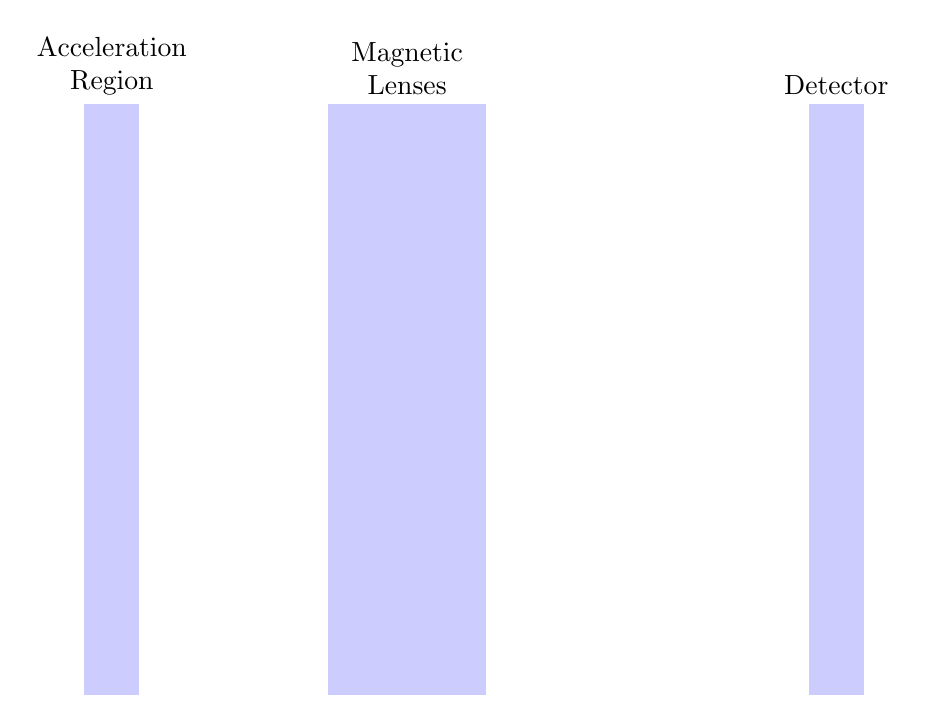
\begin{tikzpicture}
  \fill [blue!20] 
    (1.3,0.95)
    -- ++(0.7,0)
    -- ++(0,7.5)
    -- ++(-0.7,0)
      node [black, above, pos=0.5, align=center] {Acceleration\\Region}
    -- cycle
  ;
  \fill [blue!20]
    (4.4,0.95)
    -- ++(2,0)
    -- ++(0,7.5)
    -- ++(-2,0)
      node [black, pos=0.5, above, align=center] {Magnetic\\Lenses}
    -- cycle
  ;
  \fill [blue!20] 
    (10.5,0.95)
    -- ++(0.7,0)
    -- ++(0,7.5)
    -- ++(-0.7,0)
      node [black, above, pos=0.5] {Detector}
    -- cycle
  ;
  \inputdata{fig1data}
\end{tikzpicture}

  \caption{
    Simulations of the electron pulse propagation through the apparatus using the extended AG model.  
    Solid line: The spatial beam width (normalized to that at the photocathode $\Delta x_0$) with the magnetic lens strengths adjusted to ensure that the detector is at their back focal plane (Fourier plane).
    Dashed line: The case when the strength of the magnetic lenses is increased by a factor of two to focus the electron beam on the YAG scintillator detector.
  }
  \label{fig:este-sim}
\end{figure}

\ref{fig:este-sim} depicts the experimental technique used to determine directly the transverse momentum distributions (and hence $\Delta p_x$) of the laser-driven electron sources.
The primary laser radiation source for the studies is a home-built, diode-pumped and thermal-lens-shaped, femtosecond Yb:KGW oscillator\cite{berger_high-power_2008} delivering 250fs duration pulses at 1047nm and a 63MHz repetition rate (see Section \ref{sec:laser}).
This 2W average power laser is frequency doubled in a 3mm lithium triborate (LBO) crystal with 50\% efficiency to yield $\sim$200fs green pulses at 523nm (photon energy, $\hbar \omega$ = 2.37eV).
Further doubling with a cylindrical focusing geometry in a 7mm $\beta$-barium borate (BBO) crystal yields 261nm ($\hbar \omega$ = 4.75eV) UV pulses with a duration of $\sim$4ps (due to the 600fs/mm group velocity mismatch between the green and generated UV).
Both the green and UV laser pulses are focused with 30cm focal lenses onto the photocathode in a 20kV electron gun at an angle of incidence of $60(\pm5)^{\circ}$, which improves the coupling of the $p$-polarized laser radiation into the photocathode surface\cite{berger_dc_2009}.
The electron gun design is based on the that of Togawa et al.\cite{berger_dc_2009,togawa_ceb6_2007} and has an acceleration gap of 25($\pm$2)mm.
After acceleration in the DC photo-gun, the electrons pass through a set of electrostatic deflection plates to ensure that the electron beam passes, as close as possible, axially through the center of two, 6.35mm-bore, thin and round magnetic lenses with counter-propagating currents to minimize image rotation effects.
A YAG scintillator placed 27.5cm after the second magnetic lens detects the spatial electron beam profile, and its visible fluorescence is 1:1 imaged onto a CCD detector with 5.4$\mu$m pixels. 

To ensure that the transverse momentum distribution is observed, the YAG scintillator must be positioned at the back focal plane (the Fourier plane) of the lens system.
This is readily achieved by appropriate adjustment of the current $I$ in the magnetic lens coils; specifically, after determining the current required to focus the electron beam onto the scintillator, optical imaging relations together with the $I^2$ dependence of the magnetic lens strength are used to find the current that ensures that the average lens to scintillator distance equals the focal length of the lens system.
Simulation of the experimental apparatus (employing the extended AG model, see Section \ref{sec:external_forces} ), also shown in \ref{fig:este-sim}, confirms that this procedure places the YAG scintillator at the back focal plane of the lens system to within a $\pm$0.5cm error.
This simulation also confirms that for our experimental conditions (less than 5,000 electrons/pulse and $\Delta x > $ 30$\mu$m) space-charge effects do not influence the observations.
Additionally, and as expected from optical considerations, the modeling shows that the spatial beam size in the Fourier plane is independent of the incident laser spot size on the photocathode (i.e., the electron source size, $\Delta x_0$). 

\begin{figure}
  \centering
  \begin{tikzpicture}
  \inputdata{fig2data}
  \node (example) at (3.6,6.5) {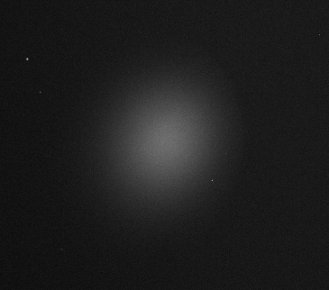
\includegraphics{fourier-020.jpg}};
  \draw [very thick, ->] (5.65,4.1) to [out=80, in=-10] (example.east);
\end{tikzpicture}

  \caption{
    Measured Fourier plane electron beam size (HWe$^{-1}$M; squares) and electron yield (circles) as a function of the incident $\sim$200fs, 523nm laser pulse energy for the 300nm-thick gold photocathode.
    The electron yield is proportional to the square of laser pulse energy (solid line) and the dependence of the beam size with the laser pulse energy fits that predicted by a zero free parameter electron heating model (solid line; dashed lines represent $\pm$10\% error in the laser spot size).
    A representative raw Fourier plane beam image is also shown.
  }
  \label{fig:gold-emission}
\end{figure}

To verify the efficacy of the experimental technique, we monitored the momentum distribution (Fourier plane spot size) for electrons emitted by 2PTE from gold using the $\sim$200fs green (523nm) $p$-polarized laser pulses.
Due to the 60$^{\circ}$ angle of incidence, the circular laser beam is focused by the 30cm focal length lens to an elliptical 50x100$\mu$m (half-width 1/e maximum (HWe$^{-1}$M) of the field) spot size on the photocathode surface.
The results, the measured Fourier plane beam size and electron yield, are displayed in \ref{fig:gold-emission} as a function of the incident laser pulse energy, corrected to account for 10\% optical loss (mainly from the uncoated vacuum system windows).

The quadratic dependence of the electron yield on pulse energy clearly indicates a two-photon emission process.
This is expected since an excitation energy of two green photons ($\hbar \omega$ = 2.37eV) will be required to overcome the reported $\phi$ = 4.69eV effective work function of a thick gold film contaminated with adsorbed water\cite{monjushiro_ultraviolet_1991} or ensure that at least the tail of the electron Fermi distribution has sufficient energy to overcome the 5.1($\pm$0.1)eV work function of a clean Au surface\cite{eastman_photoelectric_1970}.
Moreover, when $2\hbar \omega \approx \phi$, the dependence of the yield on the square of the electron's excess energy above the work function\cite{monjushiro_ultraviolet_1991} ensures that predominantly only the high energy (Boltzmann) tail of the Fermi distribution contributes to the emission.
Consequently, the observed increase in $\Delta p_x$ with incident pulse energy must be due to a heating effect; specifically, laser heating of the free electron Fermi gas as two-photon excitation is instantaneous and the $\sim$200fs green laser pulse duration excludes any coupling to the lattice which occurs on the time scale of a few picoseconds\cite{chen_semiclassical_2006}.
The solid line in \ref{fig:gold-emission} is the predicted variation derived using a simple zero free parameter model of this effect.
Using the known optical properties of gold\cite{johnson_optical_1972}, which give a reflectance $R_p$ = 0.53 and an absorption depth of 20nm, and the temperature-dependent heat capacity of a free electron Fermi gas, the model evaluates the average temperature of the laser-heated electron gas that may be two-photon excited assuming that only electrons within a few nanometers of the surface can be emitted, as the mean free path for electrons in Au is $\sim$4nm\cite{seah_quantitative_1979}.
This average electron temperature $T_e$ is then used in the AG model simulation of the experiment (\ref{fig:este-sim}) to determine the expected Fourier plane spot size on the YAG scintillator; that is, using an initial $\Delta p_x = \sqrt{m_0 k_B T_e}$.  The dashed lines indicate the expected trends for a $\pm$10\% error in the laser spot size $\Delta x_0$ incident on the gold cathode surface.
The close agreement between the data and the simulation strongly supports our interpretation of the emission mechanism and, as expected, that the effective mass of a free electron in Au is equal to the rest mass $m_0$\cite{johnson_optical_1972}.

\begin{figure}
  \centering
  \begin{tikzpicture}
  \inputdata{fig3data}
\end{tikzpicture}

  \caption{
    Number of electrons emitted per pulse as a function of the incident 261nm, UV laser pulse energy for GaSb (open squares) and InSb (filled circles): Linear efficiency dependences are shown by the solid lines.
    The laser pulse energy invariance of the Fourier plane electron beam size (HWe$^{-1}$M right axis; open squares) for GaSb and a representative raw Fourier plane beam image is also shown.
  }
  \label{fig:este-semicond}
\end{figure}

\ref{fig:este-semicond} depicts the results obtained for GaSb and InSb photocathode materials under pulsed UV (261nm) laser irradiation using the same experimental technique.
Both samples are cut from [100]-oriented polished wafers; the GaSb is undoped and the InSb is moderately $p$-type.
Prior studies\cite{gobeli_photoelectric_1965} indicate that single-photon photoemission should not possible for either semiconductor --- the effective photoemission work functions (about 4.8eV for undoped GaSb and 4.89eV for $p$-type InSb (Fermi level pinned at valence band maximum)) being greater than the 4.75eV photon energy even when the 34meV Schottky barrier suppression due to the applied 8kV/cm DC field is included\cite{dowell_quantum_2009}.
Nonetheless, for both zincblende semiconductors, significant laser-driven emission (more than expected for a single-photon field emission process) is observed with a yield nearly linearly proportional to the $\sim$4ps UV laser pulse energy.

The known optical properties of the two semiconductors\cite{aspnes_dielectric_1983} indicate a strong absorption at 261nm, with an optical absorption depth of only 7-8nm, which, based on the band structures of GaSb\cite{chelikowsky_nonlocal_1976} and InSb\cite{chelikowsky_erratum_1984}, is primarily due to promotion of electrons near the $\Gamma$ point from the valence band (heavy-hole, light-hole, and split-off bands) directly into the upper $\Gamma_8$ conduction band located at 3.77eV and 3.59eV above the valence band maximum in GaSb and InSb, respectively.
Assuming parabolic bands and an estimated effective mass $m^*$ of about 0.3$m_0$ (0.5$m_0$) for the $\Gamma_8$ conduction band in GaSb (InSb), we determine that these electrons are excited with an average excess energy (above the $\Gamma_8$ conduction band minimum) of $\sim$0.35eV ($\sim$0.41eV).
For the $\sim$0.1nJ incident UV pulse energies, $\sim40\mu$m laser spot size, and $p$-polarized reflectance of $\sim$40\% for both semiconductors at our 60$^{\circ}$ incidence angle, the photo-injected electron density is $\sim10^{18}cm^{-3}$.
At these carrier densities, which are non-degenerate for the upper $\Gamma_8$ conduction bands, we expect rapid thermalization\cite{portella_k-space_1992} and, consequently, an electron distribution with a well-populated Boltzmann tail extending above the vacuum level located at an effective work function $\phi$ of 0.99eV (1.18eV) above the $\Gamma_8$ conduction band minimum in GaSb (InSb); thus allowing for thermionic emission from this excited state as initially $\exp[\phi/(k_B T_e)] \approx 0.06$ in both semiconductors.  

Carrier cooling, primarily by longitudinal optical (LO) phonon emission, and decay out of the upper conduction band to lower states will rapidly deplete the Boltzmann tail above $\phi$, thereby curtailing the observed ESTE.
By comparison with the $\Gamma_6$ conduction band Fr\"ohlich coupling constant in GaAs, where the characteristic LO phonon emission time is 165fs for a hot electron in the $\Gamma_6$ condunction band\cite{kash_subpicosecond_1985}, we estimate that hot electrons in the upper $\Gamma_8$ conduction band of both GaSb and InSb emit a LO phonon every $\sim$200fs with an energy of 29 and 24meV, respectively.
This means that even without population decay mechanisms the temperature of the exited electron distribution $T_e$ drops at a rate of $\sim$1,600K/ps in both semiconductors.
We note that the close proximity of the lower and unconfined (in momentum space) $\Gamma_7$ upper conduction band to the $\Gamma_8$ band will likely result in a fast population decay, so that the observed ESTE process should have an intrinsic latency of much less than the $\sim$4ps UV laser pulse duration.

\ref{fig:este-semicond} also shows that the measured Fourier plane electron beam spot size for GaSb is independent of the UV laser pulse energy, as would be expected for the proposed emission process.
More significantly, using $\Delta p_x = \sqrt{m_0 k_B T_e}$ (i.e., assuming the emitted electrons have a mass $m_0$ in the semiconductor), simulation of the experiment with the extended AG model\cite{berger_semi-analytic_2010} indicates that the observed GaSb Fourier plane spot size of 0.45($\pm$0.03)mm (HWe$^{-1}$M) would be due to an electron temperature $T_e \approx$ 360K which is associated with negligible thermionic emission ($\exp[-\phi/(k_B T_e)] \sim 10^{-15}$).
On the other hand, employing a mass of 0.3$m_0$ for the electrons in GaSb allows an average electron temperature (over the $\sim$4ps laser pulse duration) of about 1,200K to be extracted using the AG model simulation --- a value much more consistent with the proposed ESTE mechanism and the expected cooling rate by LO phonon emission.
In fact, at the maximum $\sim$0.2nJ incident UV laser pulse energy up to 108 electrons/pulse could be excited into the upper $\Gamma_8$ conduction band, of which one in $\exp[\phi/(k_B T_e)] \approx$ 20,000 are above the effective 0.99eV work function, thus agreeing with the observed yield of $\sim$10$^3$ electrons/pulse (\ref{fig:este-semicond}).
We also note that the normalized transverse rms emittance $\varepsilon_{\smallT}$ of this UV laser-driven ultrafast GaSb electron source is more than a factor of two less than that expected from a standard Cu photocathode ($\phi$ = 4.31eV and assuming $\Delta p_x = \sqrt{m_0 ( \hbar \omega - \phi ) / 3 }$, where $\hbar \omega$ is the incident photon energy\cite{dowell_quantum_2009,jensen_emittance_2010}) irradiated at the same 261nm wavelength.

Very similar results are observed with the $p$-type InSb photocathode except that the Fourier plane spot size is 30-40\%  larger and the electron yield is a factor of 1.7 higher.
The increased rms transverse momentum for the same ESTE process is consistent with the larger $\sim$0.5$m_0$ effective mass of the upper $\Gamma_8$ conduction band in InSb, the expected higher initial temperature of the electron distribution, and the marginally slower cooling process associated with the lower 24meV LO phonon energy.
The resultant higher average electron temperature $T_e$ also contributes to the increased electron yield that is likely further enhanced by a larger absorption into the upper $\Gamma_8$ conduction band (due to its larger effective mass) and a 4\% lower $p$-polarized reflectance for the 60$^{\circ}$ incident UV laser radiation\cite{aspnes_dielectric_1983}. 

The dependence of $\Delta p_x$ on $m^*$ is readily explained through a consideration of energy and momentum conservation in transmission across a boundary with a potential step associated with the effective photoelectric work function $\phi$.
Inside the material, an electron with an energy $E$ greater than $\phi$ has a maximum momentum of $\sqrt{2 m^* (E-\phi) }$ parallel to the boundary if it is to be emitted.
As this momentum component is conserved in emission from the material surface into the vacuum, the rms transverse momentum $\Delta p_x$ of the electron source clearly must scale with $\sqrt{m_*}$ as observed in the experiment.
This is, of course, the \textit{sine qua non} of angle-resolved photoemission studies\cite{himpsel_angle-resolved_1983} where determination of the electron emission angle and energy allows the effective mass parallel to the sample surface to be determined.
We note that the electron effective mass also causes the narrow emission cone reported for $p$-type GaAs(100) negative electron affinity photocathodes\cite{liu_narrow_2005}, where surface cesiation lowers the vacuum level below the $\Gamma_6$-valley minimum ($m^* = 0.067m_0$)  to allow for direct emission of electrons excited into the conduction band.
For direct single-photon photoemission, we would therefore also expect to require that the expression describing the rms transverse momentum to be written as $\Delta p_x = \sqrt{m^* ( \hbar \omega - \phi ) / 3 }$.
Efforts are currently underway to determine if this is indeed the case using a variety of metal photocathodes and the $\sim$ps, 261nm laser radiation source. 
